%!TEX root = ../../root.tex

The idea of GANs is that we are training the generator on data that is produced by an adversary. This is an example of a more general concept called \emph{adversarial training}, in which the data samples that are used for training are called \emph{adversarial examples}.

They are not just useful for training more accurate models, but they can also be used \emph{maliciously}, to fool a model with the sole purpose of making it fail.

The existence of adversarial examples for a model, meaning examples over which the model fails when it is not expected to do so, can be an indicator of poor \emph{robustness} of the model: if we can find such adversarial examples it means that our trained model is not very robust.

\paragraph{Examples}

Suppose we have a model trained to recognize traffic signs, and that it is able to recognize regular stop signs. Now, on the stop signal in \cref{fig:malicious} was applied some kind of perturbation, in the form of two writings, in a very specific configuration of color and position. The model fails, recognizing the sign as a speed limit sign, instead of a stop sign. This particular adversarial example was found by a generator that has been trained specifically to have the original classifier misclassify the stop sign.

\begin{figure}[H]
	\centering
	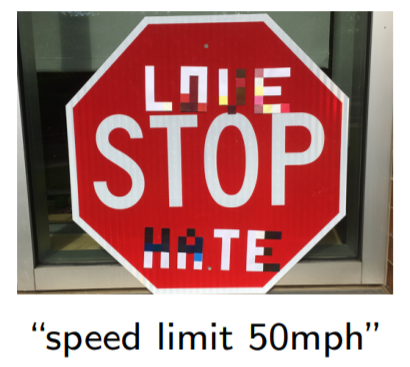
\includegraphics[width=.4\textwidth]{13/7_17}
	\caption{An example of malicious application. }\label{fig:malicious}	
\end{figure}

In \cref{fig:schoolbus} we can see two pictures of a school bus. They are the same picture to a human observer, but actually the second is the result of perturbation being applied the first one, in order to get a classifier to misclassify it as something else, an ostrich in this example. Perturbations added to the original sample are usually explicitly optimized to be imperceptible.

\begin{figure}[H]
    \centering
    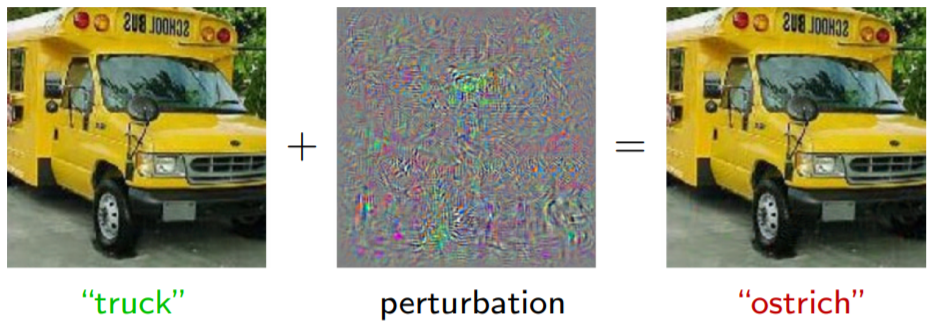
\includegraphics[width=.7\textwidth]{figures/13/8_17.png}
    \caption{Imperceptible adversarial attack.}
    \label{fig:schoolbus}
\end{figure}

\paragraph{Perception}
Let's now see how to construct undetectable adversarial examples.

An attack is said to be \emph{undetectable} if it can not be perceived as such. However this is only a loose definition, and we need a \emph{metric} or \emph{measure} that quantifies how good we are at perceiving stuff. This measure should:
\begin{itemize}
	\item capture the \emph{noticeability} of the attack, i.e. how much the attack is noticeable by a perceiver;
	\item be \emph{minimizable}, so we can explicitly construct undetectable adversarial examples: if we define the ``optimal'' adversarial example to be the one that makes this measure as small as possible, then the adversarial example will be as little noticeable as possible.
\end{itemize}

The choice of such measure will depend on the domain and on the task. 

\begin{figure}[H]
	\centering
	\subfloat[Classification at pixels level.]{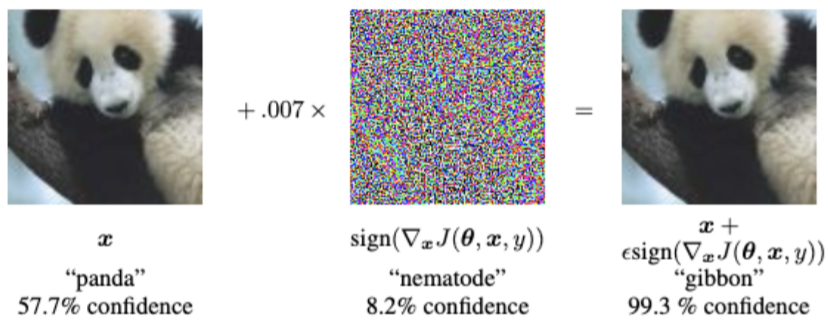
\includegraphics[width=.7\textwidth]{13/9_17_panda}} \\
	\subfloat[Classification of pose of a 3D shape.]{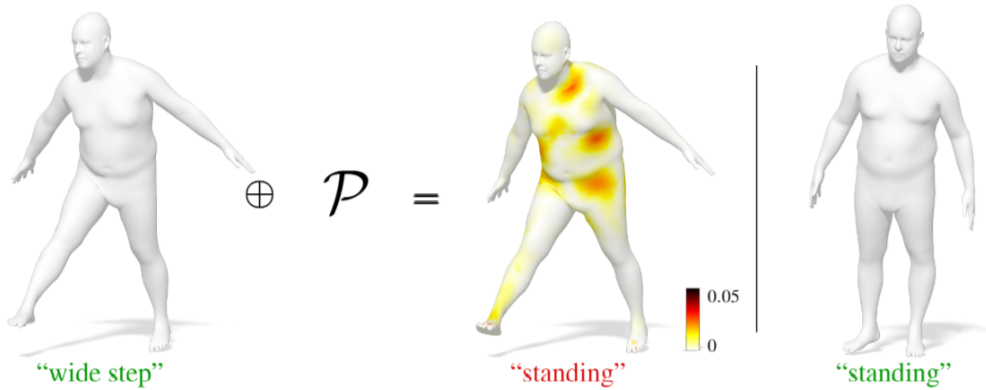
\includegraphics[width=.7\textwidth]{13/9_17_3D_shape}}
	\caption{Different perturbations for different tasks.}
\end{figure}

\paragraph{Types of attacks}

We can classify attacks based on how much information we have on the model that we are trying to attack.
\begin{itemize}
    \item \textbf{Black-box attack}. \\
    We are given a trained deep neural network but we do not know anything about the network, we can just give input samples to the network and observe the output.
    \item \textbf{Gray-box attack}. \\ 
    We have access to some \emph{partial} information about the model \textit{e.g.} only the features, or the architecture, etc.
    \item \textbf{White-box attack}. \\ 
    We have complete access to the network.
\end{itemize}
We will see \emph{white box attacks} because it has been shown that it is possible to train a \emph{substitute model}, with black box access to the target model that we would like to attack, such that the substitute gives the same input-output pairs. Then we can study attacks the substitute model with a white box approach and then transfer the attack to the original black box target.
\\

\textbf{Note.} When we attack a neural network or learning based model in general, we \emph{cannot change its parameters}. This is not the purpose of the attack: instead, what we want to do is, given a trained network, we want to find a properly crafted sample, possibly undetectable, that the trained network will misclassify. There is no training involved in attacks, since there is no modifying the network parameters. If that was the case, we could trivially mess with them and make it compute garbage.

\subparagraph{Targeted attacks}
When performing \emph{targeted} attacks, we are given a classifier $C$ and some input sample $\mathbf{x}$ and a \emph{target class} $t$, meaning the class towards which we want to misclassify. For example, we might want a self-driving car to misclassify a stop sign as a speed limit sign, and in this case this would be a targeted attack, in which the target is the class `speed limit sign'. 

To find an adversarial example for a targeted attack, we solve the following minimization problem:
\begin{align}
	\min_{\mathbf{x'} \in [0,1]^n}& \|\mathbf{x} - \mathbf{x'}\|^2_2 \\
	&\text{s.t. } C(\mathbf{x'}) = t
\end{align}
so we are trying to look for a new image $\mathbf{x'}$ that is as close as possible to the original one (being imperceptible) and also such that this new image $\mathbf{x'}$ will be classified as the target class. 
\\

\textbf{Note.} $C$ is not directly the deep neural network, because the neural network does not output a predicted class, but a probability distribution over all the classes. Usually $C$ is the $\argmax$ of the output of the network.
\\

This kind of optimization problem is very difficult since the constraint is highly nonlinear, so we can relax the problem by substituting the constraint with a penalty represented by the cross-entropy loss $L$:
\begin{equation}
	\min_{\mathbf{x'} \in [0,1]^n} \|\mathbf{x} - \mathbf{x'}\|^2_2 + cL(\mathbf{x'}, t).
\end{equation}
We still want $\mathbf{x'}$ to be misclassified by the network as $t$, but we are not imposing a hard constraint any longer, but instead a tradeoff by $c$.

As $c$ goes to zero, the problem is not really interesting any longer since the $\mathbf{x'}$ that satisfies $\|\mathbf{x} - \mathbf{x'}\|^2_2$ is trivially $\mathbf{x}$. 

On the other hand, as $c$ goes to infinity then $\|\mathbf{x} - \mathbf{x'}\|^2_2$ is not considered any longer, and the perturbation applied will be very noticeable, so we want to find a good balance between the two terms, like it is always the case when there is a tradeoff. In this case, one approach is choosing the right value for $c$ via \emph{line search} algorithms.
\\

A more general approach has been proposed. Instead of using the $L_2$ norm as a distance between adversarial sample and original sample, we can use a more generic notion of distance that depends on the specific problem, and we can explicitly talk about the perturbation $\delta$:
\begin{align}
	\min_{\delta \in [0,1]^n}& d(\mathbf{x}, \mathbf{x}+\delta) \\
	&\text{s.t. } C(\mathbf{x}+\delta) = t.
\end{align}
We are optimizing over the space of possible perturbations $\delta$ to be added to the original sample. In particular, we are seeking the $\delta$ that is the closest possible to the original sample $\mathbf{x}$ in terms of the distance function.

Now, it has been proposed to replace the hard constraint with an inequality constraint:
\begin{align}
	\min_{\delta \in [0,1]^n}& d(\mathbf{x}, \mathbf{x}+\delta) \\
	&\text{s.t. } f(\mathbf{x}+\delta) \leq 0
\end{align}
in which $f$ is a function such that
\begin{equation}
    C(\mathbf{x} + \delta) = t ~~ \iff ~~ f(\mathbf{x} + \delta) \leq 0.
\end{equation}
Several definitions are possible for such a function $f$.

Then, as the previous approach we can turn the constraint into a penalty:
\begin{equation}
	\min_{\delta \in [0,1]^n} d(\mathbf{x}, \mathbf{x}+\delta) + cf(\mathbf{x}+\delta).
\end{equation}

A possible instantiation of this problem is the following:
\begin{equation}
	\min_{\delta \in [0,1]^n} \|\delta\|_p + c(\max_{i \neq t} \left\{ F(\mathbf{x}+\delta)_i \right\} - F(\mathbf{x}+ \delta)_t)^+
\end{equation}
in which:
\begin{itemize}
    \item The first term is the distance function. It is just the $L_p$ norm of the perturbation $\delta$. If the perturbation has small norm, then the original and adversarial samples will necessarily be close.
    
    \item The second term is a possible definition of the function $f$, actually one that has been shown to work well in practice. Let's see the various terms one by one.
    \begin{itemize}
        \item $F: \vb{x} \to [0, 1]^k$ is the neural network that takes as input a value $\mathbf{x}$ and outputs a probability distribution over the $k$ classes.
        \item So, $F(\mathbf{x}+ \delta)_t$ is the value of the (predicted) probability of the adversarial sample to be of class $t$.
        \item Instead, $\max{F(\mathbf{x}+\delta)_i : i \neq t}$ is the value of the probability of the ``strongest class'' (the one the network $F$ has has more confidence predicting) that is not our target class.
        \item The $()^+$ notation is just a shorthand notation for $(\cdot)^+ = \max(\cdot, 0)$.
    \end{itemize} 
\end{itemize}

This penalty is then trying to look for the perturbation $\delta$ such that when we give $\mathbf{x} + \delta$ to the network, then the probability of class $t$ is the biggest while the probability of all other classes, considered one by one in order of ``confidence'', is suppressed.
\begin{figure}[H]
	\centering
	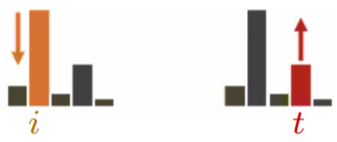
\includegraphics[width=.2\textwidth]{13/12_17}
	\caption{Intuition of the definition of $f$.}\label{fig:intuition}	
\end{figure}

\subparagraph{Untargeted attacks}

We perform an \emph{untargeted attack} when we just want a sample to be misclassified with no preference for the target class. 

This can be done very efficiently. Suppose we are given an input $\mathbf{x}$ with a ground-truth label $\ell$. The network was trained by minimizing the cross-entropy loss $\mathcal{L}(\cdot, \cdot)$, and to misclassify $\mathbf{x}$ it means to increase the loss $\mathcal{L}(\mathbf{x}, \ell)$. Then, we can define our adversarial example as
\begin{equation}\label{eq:untargeted}
	\mathbf{x'} = \mathbf{x} + \epsilon \underbrace{sign(\nabla \mathcal{L}(\mathbf{x}, \ell))}_{\text{perturbation}}
\end{equation}
which adds a \emph{perturbation} that maximizes the cost.
\\

\textbf{Note.} The gradient is computed wrt to the sample $\vb{x}$, not the model's paramaters. So by increasing $\vb{x}$ along the direction of the gradient of the loss \emph{in sample space}, we are effectively increasing the loss by the biggest possible amount.
\\

The parameter $\epsilon$ decides how small the perturbation should be. We can iterate \cref{eq:untargeted} by performing several ``perturbation steps'':
\begin{equation}
	\mathbf{x'}_{(i)} = \mathbf{x'}_{(i-1)} + \alpha \ sign\left( \nabla \mathcal{L}(\mathbf{x'}_{(i-1)}, \ell) \right), \qquad \vb{x}'_{(0)} = \vb{x}.
\end{equation}
The parameter $\alpha \ll \epsilon$ is very small, so that we have finer control on the perturbation process. 

To prevent the attack from becoming too noticeable, we add a \emph{clipping} operationl. After each perturbation step, we want to make sure that the resulting sample did not go too far away from the original sample. In particular, the \emph{clip} operation projects the sample back into an $\epsilon$-neighborhood of the original sample $\vb{x}$.
\begin{equation}
	\mathbf{x'}_{(i)} = clip_{\epsilon} \left(\mathbf{x'}_{(i-1)} + \alpha \ sign\left( \nabla \mathcal{L}(\mathbf{x'}_{(i-1)}, \ell) \right)\right)
\end{equation}

We can notice how the perturbation process might be optimized further by assigning different weights to each component of the sample, instead of adding the same perturbation $\alpha$ to every one of them. However, this method was designed to be efficient, and in fact it can be done with just one backpropagation step, plus some other far less costly operations like clipping, so it is indeed very efficient. Nevertheless, this simple attack can work well in practice.


\paragraph{Vulnerability}

If we are able to produce adversarial examples then we can use them to train our model, improving the robustness of the attacked learning model.

However, it has been shown that for an arbitrary classifier, no matter how robust we try to make it, there will always exist in theory small adversarial perturbations that make the classifier fail. This means that there is a maximal achievable robustness.

The main observation is that, very often, a trained classifier will learn decision boundaries that are \emph{very close} to the data points. This means that we can move them just by a little bit, and then suddenly they will get to the other side of the boundary which means that they will be misclassified.
\begin{figure}[H]
	\centering
	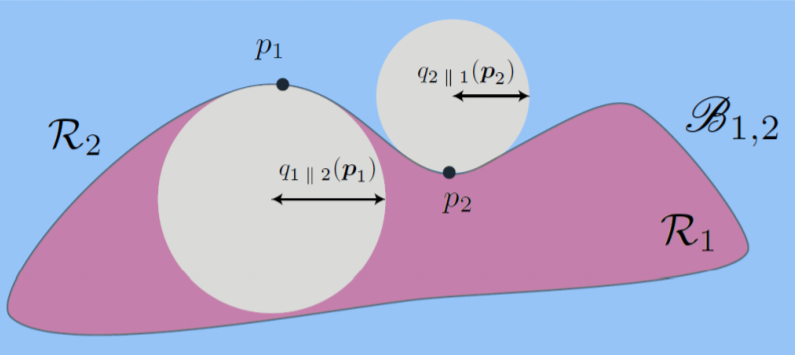
\includegraphics[width=.8\textwidth]{13/15_17}
	\caption{(Nonlinear) Decision boundary for an arbitrary learning model.}\label{fig:boundary}	
\end{figure}
The success rate of the attacks has been found to be related to the \emph{curvature} of the decision boundary of a neural network classifier. With this mathematical formulation we can quantify the robustness as a function of this curvature.
\\

\paragraph{Universal perturbations}

So far we have always expressed our attacks in terms of a specific sample $\vb{x}$ that we wanted the attacked network to misclassify. However, it would be far mor drastic if we could make a network fail almost on every sample.

In an impactful work of a few years ago, the existence of \emph{universal perturbations} has been shown.
They are types of perturbations that, for a given attacked network and a large set of samples $\vb{x}$, are adversarial for the entire set, making them \emph{universal}.

\begin{figure}[H]
    \centering
    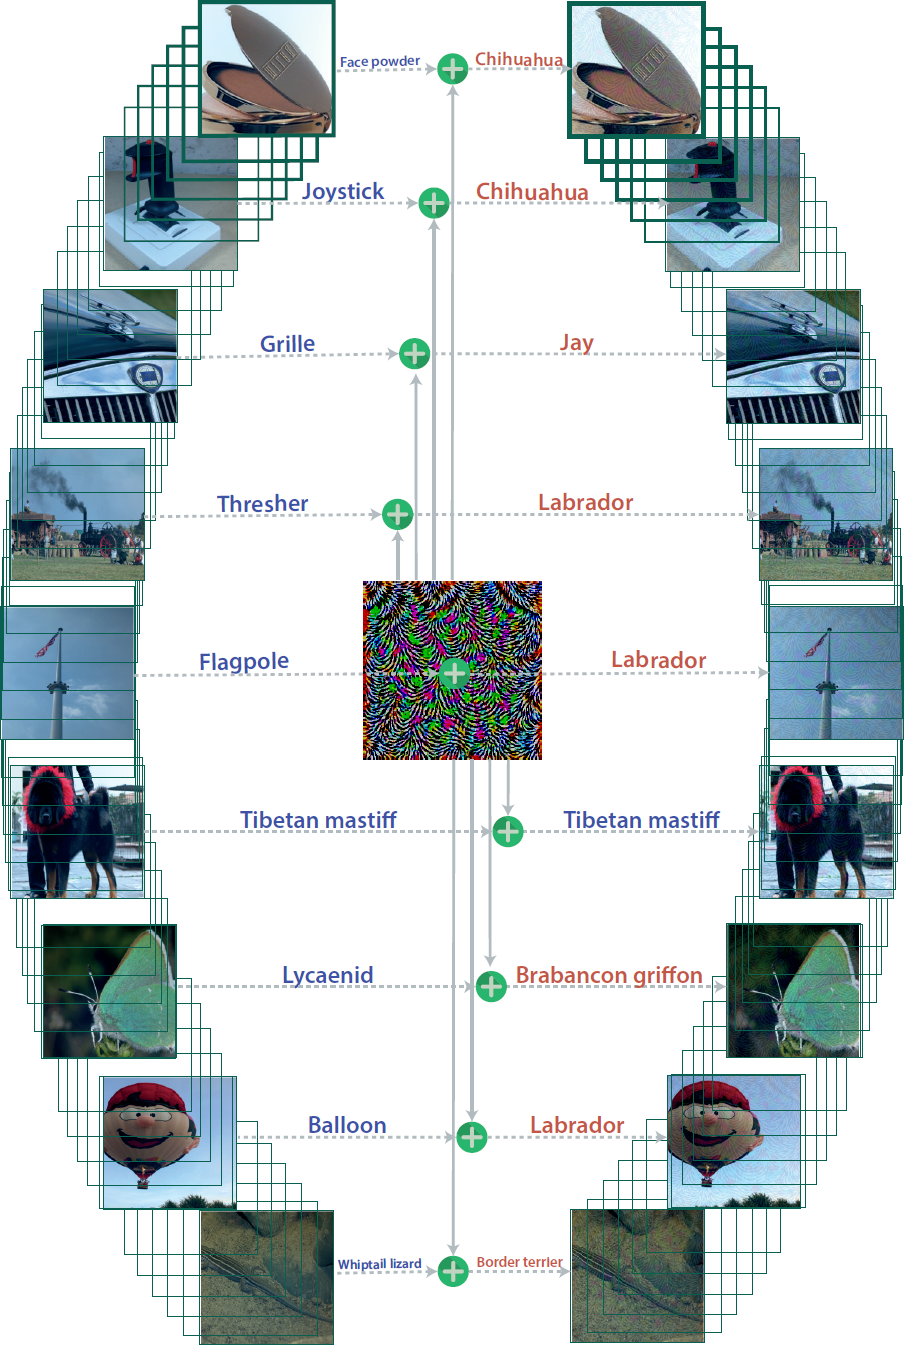
\includegraphics[width=.7\textwidth]{figures/13/universal.png}
    \caption{The perturbation in the center misclassifies all the images except for the dog.}
\end{figure}

\paragraph{Closing remarks}

Adversarial training can also be phrased on non-Euclidean domains like surfaces, graphs, point clouds and other non-Euclidean structures. 
When we deal with this kind of geometric domains the notion of what is \emph{noticeable} is different than what we had with images, and requires a careful definintion. Also, when defining an attack we can take into consideration the domain itself, beside the data defined over it. For example, we could add or remove edges or, if we were dealing with a point cloud, we could add or move points in space.  

There is a whole branch of adversarial machine learning that deals with \emph{adversarial defense}: methods and techniques to shield learning models from adversarial attacks. Adversarial training is one such method.